% =====================================================================
%  Neural Demodulation of Hardware-Captured PSK and Star-QAM Waveforms
%  Under a Provable Memorisation Bound
%
%  Target: IEEE Access
%
%  SUBMISSION SWAP
%  IEEE Access supplies ieeeaccess.cls, which is not in a standard
%  MiKTeX/TeX Live installation. This file uses IEEEtran in journal mode so
%  it compiles today. At submission, download the official IEEE Access
%  template and change the \documentclass line below. Nothing else changes.
%
%  OUTSTANDING BEFORE SUBMISSION
%   1. refs.bib entries were written from working knowledge. VERIFY EVERY
%      ONE against IEEE Xplore -- volumes and pages especially -- and add DOIs.
%   2. Section II (Related Work) has marked slots awaiting the recent
%      literature you are collecting.
%   3. Author block, affiliations, acknowledgment and biographies are
%      placeholders.
%   4. Fig. 1: relabel the five boards individually as B1-B5.
% =====================================================================

\documentclass[journal]{IEEEtran}   % SUBMISSION SWAP -> {ieeeaccess}

\usepackage{graphicx}
\usepackage{amsmath}
\usepackage{amssymb}
\usepackage{booktabs}
\usepackage{multirow}
\usepackage{cite}
\usepackage[hidelinks]{hyperref}
\usepackage{url}

\graphicspath{{figures/}}
\newcommand{\SER}{\mathrm{SER}}

% ---------------------------------------------------------------------
% Draft notes. Unwritten sections must be VISIBLE in the PDF: a LaTeX
% comment renders as nothing, so a section awaiting content looks broken
% rather than pending. Set \draftfalse before submission and every note
% disappears; nothing else changes.
% ---------------------------------------------------------------------
\newif\ifdraft
\drafttrue          % <<< SET TO \draftfalse BEFORE SUBMISSION
\newcommand{\todonote}[2]{%
  \ifdraft
    \par\medskip\noindent
    \fbox{\parbox{0.94\columnwidth}{\footnotesize
      \textbf{[TO WRITE --- #1]}\\[2pt]#2}}%
    \par\medskip
  \fi}

\begin{document}

\title{Neural Demodulation of Hardware-Captured PSK and Star-QAM Waveforms
Under a Provable Memorisation Bound}

\author{
  \IEEEauthorblockN{Author One, Author Two}%
  \thanks{The authors are with the Department of [Department],
  [Institution], [City], [Country] (e-mail: [corresponding author]).}%
  \thanks{Dataset, trained models and analysis code are available at
  [repository URL].}%
}

\markboth{IEEE Access}{M.K.H Nabil \MakeLowercase{\textit{et al.}}:
Neural Demodulation Under a Provable Memorisation Bound}

\maketitle

% =====================================================================
\begin{abstract}
Learned receivers are commonly evaluated on data whose transmitted sequence is
short and periodic, which allows a sufficiently expressive model to reproduce
the sequence from context rather than demodulate the waveform. We present a
hardware dataset and a receiver design in which this failure mode is excluded by
construction. Waveforms were captured from five physically distinct
communication trainer boards across BPSK, QPSK and a four-phase two-amplitude
star 8-QAM constellation, yielding 43 oscilloscope records and 154{,}628
labelled symbols. Ground-truth labels are obtained by coherent averaging of the
transmitted waveform rather than from the transmitter's configuration, and are
verified independently: all sixteen BPSK captures reproduce the board's 63-bit
maximal-length sequence exactly, and a single memoryless mapping explains three
distinct QPSK data words simultaneously ($p < 5\times10^{-5}$). Because the
transmitted sequence has linear order six, any six consecutive bits determine
the seventh; we therefore restrict the receiver's input to at most five bits,
making prediction-from-context impossible rather than merely improbable. A
21{,}000-parameter convolutional receiver operating on the raw passband waveform
attains symbol error rates statistically indistinguishable from a blind
matched-filter receiver across all three modulations, while receiving neither
the carrier frequency, the pulse shape, nor the constellation geometry. Holding
out an entire data word costs $0.005$ in symbol error rate relative to a random
split, and on that split both a shuffled-label control and a signal-free
positional control remain at chance. We additionally report two negative
results: a constellation-geometry loss term does not improve error rate, and a
widely suggested carrier-sensitivity comparison does not survive measurement.
\end{abstract}

\begin{IEEEkeywords}
Neural receiver, demodulation, deep learning, physical layer, hardware dataset,
maximal-length sequence, memorisation, symbol error rate, quadrature amplitude
modulation.
\end{IEEEkeywords}

% =====================================================================
\section{Introduction}
\IEEEPARstart{L}{earning}-based receivers recover digital modulation from
sampled waveforms without an explicitly specified signal
model~\cite{oshea2017intro,dorner2018ota,ye2018power}. A recurring difficulty in
evaluating such systems is that the transmitted data is frequently a short
pseudorandom sequence repeated many times. When that is so, a model with
sufficient temporal context can predict the next symbol from preceding symbols
alone, without extracting any information from the waveform. The reported error
rate then measures sequence memorisation rather than demodulation, and held-out
evaluation does not detect this if the same short sequence appears in both
partitions.

This paper takes the position that the property should be excluded structurally
rather than argued empirically. The transmitters studied here emit a
maximal-length sequence of linear order six. For such a sequence, any six
consecutive bits determine the seventh exactly, while any five do not. A
receiver whose input contains at most five bits therefore cannot perform
prediction-from-context, irrespective of its capacity, its training procedure,
or the quantity of data available to it. We enforce this by limiting the
receiver's input window, so that the bound is a property of the data presented
to the network rather than of its architecture, and can be verified by
inspection.

The contributions are as follows.

\begin{enumerate}
\item A hardware dataset of 43 dual-channel oscilloscope captures from five
physically distinct trainer boards, spanning BPSK, QPSK and a two-ring star
8-QAM constellation, with a per-record verification protocol and full
provenance (Section~\ref{sec:dataset}).
\item A ground-truth procedure based on coherent averaging of the transmitted
waveform, with two independent confirmations that the recovered labels are
correct (Section~\ref{sec:groundtruth}).
\item A receptive-field bound that makes sequence memorisation impossible,
stated as a proof and confirmed empirically by the absence of any gap between a
random split and a leave-one-pattern-out split (Sections~\ref{sec:bound}
and~\ref{sec:generalisation}).
\item A characterisation of the boards' own demodulators, including a lock
threshold reproducing across all five units, and evidence that self-consistency
is an invalid criterion for demodulator lock (Section~\ref{sec:hardware}).
\item Two negative results, reported because they bear directly on claims made
elsewhere in this literature: a constellation-geometry loss term does not
improve error rate, and a blind classical receiver's dependence on carrier
knowledge does not constitute a practical disadvantage at any observation length
tested (Sections~\ref{sec:geometry} and~\ref{sec:limitations}).
\end{enumerate}

We make no claim of improved error-rate performance. The learned receiver
attains parity with a blind classical receiver; the contribution is that it does
so without being supplied the carrier frequency, the pulse shape, the
constellation geometry or the decision boundaries, and that it provably cannot
have obtained its result by memorisation.

% =====================================================================
\section{Related Work}
\label{sec:related}

\subsection{Learned physical-layer processing}
Learned physical-layer processing has been demonstrated for end-to-end
autoencoder transceivers~\cite{oshea2017intro}, for systems trained over the
air~\cite{dorner2018ota}, and for joint channel estimation and
detection~\cite{ye2018power}. Modulation classification from sampled in-phase
and quadrature data has received particular attention, along with the associated
public datasets~\cite{oshea2018classification}.

\todonote{recent neural demodulation, 2--3 paragraphs}{%
Add work from the last two to three years on neural demodulation and neural
receivers. For each: one sentence on what it does, one on how it differs here.
The organising axis should be \emph{what each system is given}---carrier
frequency, symbol timing, pulse shape, constellation---because that is the axis
on which this paper positions itself (Section~\ref{sec:limitations} states
exactly what ours receives). Close the subsection by noting that these systems
are evaluated on held-out partitions without a structural bound on context.}

\subsection{Evaluation validity and memorisation}
This paper's premise is that held-out evaluation is insufficient when the
transmitted sequence is short and periodic. Related concerns are long-standing
in machine learning generally---train/test contamination, and models that
exploit dataset artefacts rather than the intended signal---but the specific
failure considered here is narrower: the test sequence itself is predictable
from its own past, so a model with sufficient context can reach a low error rate
without demodulating.

\todonote{evaluation validity, 1--2 paragraphs}{%
Add any prior work in learned communications that addresses train/test
contamination, sequence memorisation, or evaluation protocol. Two outcomes are
both acceptable and should be stated plainly:
\emph{(i)} if such work exists, position ours as the first to bound receiver
context below the linear complexity of the test sequence rather than argue the
point empirically;
\emph{(ii)} if little exists, say so directly---that absence is itself part of
the motivation, and is a stronger opening than a padded list. Do not manufacture
citations to fill this subsection.}

\subsection{Hardware-captured RF datasets}
Public RF datasets are commonly synthesised, or captured from a small number of
transmitters with ground truth asserted from the transmitter's configuration
rather than measured from the emitted waveform. The distinction matters here:
Section~\ref{sec:dataset} shows a case in which the configured data word is
\emph{not} a reliable statement of the transmitted symbol sequence, and
Section~\ref{sec:groundtruth} obtains labels by measurement instead.

\todonote{hardware RF datasets, 1--2 paragraphs}{%
Add existing hardware-captured RF datasets. For each, record the number of
physical devices and---most importantly---whether ground truth is
\emph{asserted} from the transmitter configuration or \emph{measured} from the
waveform. That column is where our contribution sits; a small comparison table
would carry it well if three or more comparable datasets exist. Note our device
count honestly (five) alongside theirs.}

\subsection{Classical receiver theory}
Classical treatments of the receiver functions replaced by learned
systems---carrier recovery, timing recovery, matched filtering and
detection---are given in~\cite{proakis2007digital} and~\cite{mengali1997sync}.
The timing-error detector referenced in Section~\ref{sec:limitations} is due
to~\cite{gardner1986ted}. Properties of maximal-length sequences, including the
linear recursion exploited in Section~\ref{sec:bound}, are standard and are set
out in~\cite{golomb1982shift}.

% =====================================================================
\section{Experimental Setup and Dataset}
\label{sec:dataset}

\subsection{Apparatus}
Signals were captured from MCM31/EV communication trainer boards using a
two-channel digital oscilloscope, shown in Fig.~\ref{fig:setup}. Channel~1
observes TP-20, the modulated output, and channel~2 observes TP-9, the board's
own recovered data. The two are acquired simultaneously so that network input
and hardware baseline originate from a single record. Acquisition is externally
triggered from the board's symbol clock at TP-1.

\begin{figure*}[!t]
\centering
% Printed at 0.80\textwidth rather than full width. The source photograph is
% 1280 px across, which is 179 dpi at full text width -- below the 220 dpi IEEE
% asks for on photographs -- and 223 dpi at this width. Scaling an image down
% raises its effective resolution; scaling it up would not add information.
% If a higher-resolution original of the photograph becomes available, restore
% width=\textwidth.
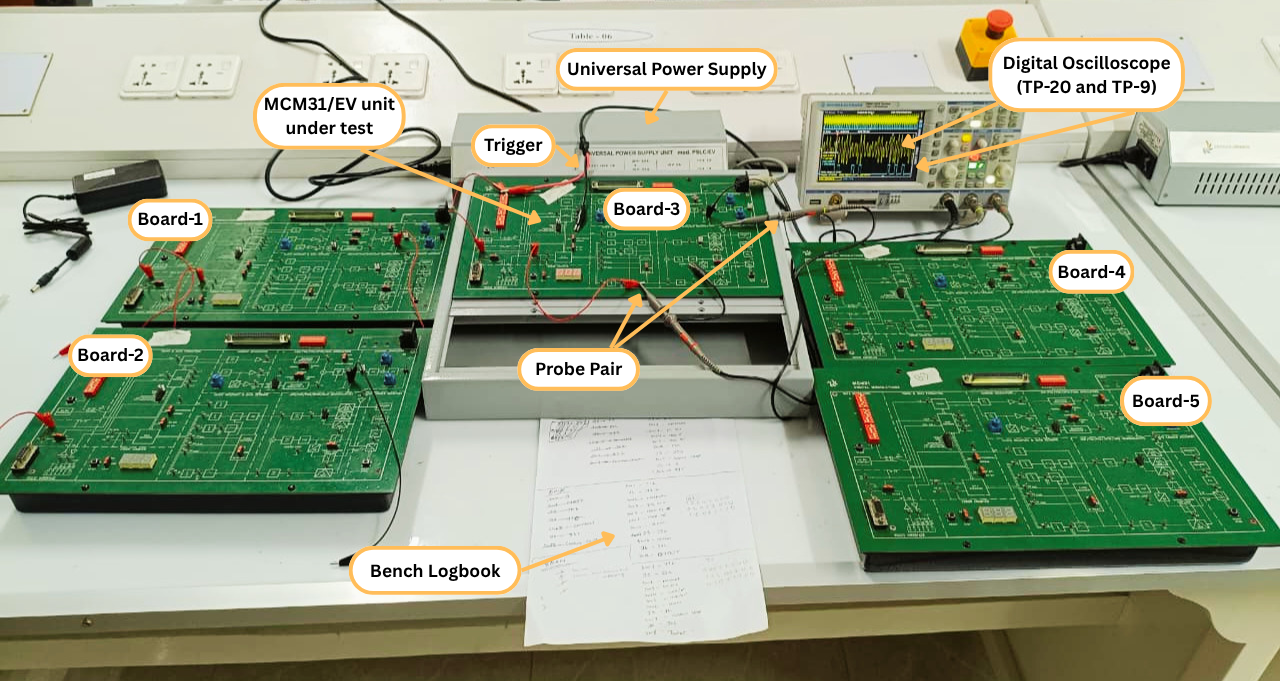
\includegraphics[width=0.80\textwidth]{fig0_setup.png}
\caption{Measurement bench. The five MCM31/EV trainer units, labelled Board-1 to
Board-5, correspond to boards B1--B5 in Table~\ref{tab:perfold} and
Fig.~\ref{fig:lock}. One unit is under test at a time, powered from a shared
supply, with the oscilloscope probing TP-20 and TP-9 simultaneously and
triggered externally from TP-1. Attenuator positions and switch settings were
photographed before and after every session.}
\label{fig:setup}
\end{figure*}

Acquisition parameters were fixed for every record and are given in
Table~\ref{tab:acq}. The time base was chosen so that each record contains at
least 57 repetitions of the longest data word, which is what makes the coherent
averaging of Section~\ref{sec:groundtruth} effective. A shorter time base was
evaluated and rejected: it yields too few repetitions for a stable
signal-to-noise estimate.

\begin{table}[!t]
\caption{Acquisition and signal parameters. All values were measured from the
captured records rather than taken from the equipment specification.}
\label{tab:acq}
\centering
\small
\begin{tabular}{ll}
\toprule
Parameter & Value \\
\midrule
Sample rate & $87{,}260$~Sa/s \\
Samples per record & $523{,}600$ \\
Record duration & $6.0004$~s \\
Channel 1 & TP-20, modulated output \\
Channel 2 & TP-9, recovered data \\
Trigger & external, from TP-1 \\
\midrule
Carrier & $1199.91$~Hz \\
Symbol rate & $599.955$~baud \\
Carrier cycles per symbol & $2$ (exact) \\
Samples per symbol & $145.44$ \\
\midrule
BPSK data source & on-board 63-bit m-sequence \\
QPSK, 8-QAM data source & 24-bit configurable words \\
\bottomrule
\end{tabular}
\end{table}

The carrier is coherent with the symbol clock at exactly two cycles per symbol.
This is the property that permits coherent averaging: the passband waveform
repeats exactly at the word period, so averaging over repetitions suppresses
noise without distorting the signal.

\subsection{Units under test}
Ten units were sourced. Five were functional; five were excluded following
individual inspection, in each case because the on-board data generator had
failed, either in the sequence-load latch or in the pseudorandom generator
itself. On such a unit the modulator receives no data and TP-20 carries an
unmodulated carrier: the coherent template contains all of its energy in the
carrier bin and none in the sidebands, and no usable waveform exists to capture.
All results below therefore rest on five boards, and leave-one-board-out is a
five-fold evaluation.

\subsection{Per-record verification}
Every record was subjected to the battery of checks in Table~\ref{tab:checks}
before admission to the corpus. The battery is not decorative: it rejected
records during the campaign and each rejection corresponded to a real
configuration fault.

\begin{table}[!t]
\caption{Per-record verification battery. Every record in the corpus passes
every check except where noted in Section~\ref{sec:dataset}-D.}
\label{tab:checks}
\centering
\small
\begin{tabular}{clc}
\toprule
\# & Check & Pass condition \\
\midrule
1  & Channel count            & 2 channels present \\
2  & Sample count             & $520{,}000$--$526{,}000$ \\
3  & Duration                 & $5.99$--$6.01$~s \\
4  & Sample rate              & $87{,}000$--$87{,}500$~Sa/s \\
5  & Quantisation levels      & $\geq 90$ distinct \\
6  & Carrier (4th power)      & $1199.5$--$1200.5$~Hz \\
7  & Word-period repetition   & $r \geq 0.95$ \\
8  & Coherent-template SNR    & $\geq 15$~dB \\
9a & Same word, two records   & similarity $\geq 0.99$ \\
9b & Constellation fingerprint & matches the expected word \\
9c & Different words          & similarity $< 0.99$ \\
10 & TP-9 agreement           & logged, not gating \\
\bottomrule
\end{tabular}
\end{table}

Checks 9a--9c deserve comment. Check~9a compares two records of the same
configured word and detects a failure to reload the transmitter between
captures. Check~9b compares the multiset of per-constellation-point occupancy
counts against the value predicted by the configured word; it is invariant to
constellation rotation and to the mapping between transmitter configuration and
transmitted symbol, and therefore identifies the loaded word without assuming
that mapping. Check~9c is the converse and is required for held-out words, each
of which is captured only once: two \emph{different} configured words must not
produce the same waveform. Neither 9a nor 9b detects a stale word in that case,
because words designed to cover the full constellation share a fingerprint by
construction.

Check~9c must be evaluated on the \emph{signed} similarity. Two words that are
bitwise complements produce waveforms that are exact negations of one another,
and an unsigned similarity reports these as identical when they are merely
antipodal.

\subsection{Corpus}
The corpus comprises 43 records: fifteen from board~B1 (seven main-campaign
records and eight additional data words held out for evaluation) and seven from
each of B2--B5. Segmentation at the symbol rate yields $154{,}628$ labelled
symbols, distributed as in Table~\ref{tab:dataset}. Coherent-template SNR across
the accepted corpus is $22.7$--$43.2$~dB, median $30.2$~dB.

\begin{table}[!t]
\caption{Dataset composition. \emph{Words} counts distinct configured bit
patterns; \emph{independent} accounts for the antipodal equivalence described in the text.
}
\label{tab:dataset}
\centering
\begin{tabular}{lrrrr}
\toprule
Modulation & Records & Symbols & Words & Independent \\
\midrule
BPSK  & 16 & 57{,}536 & 2 & 2 \\
QPSK  & 12 & 43{,}152 & 3 & 3 \\
8-QAM & 15 & 53{,}940 & 6 & 5 \\
\midrule
Total & 43 & 154{,}628 & & \\
\bottomrule
\end{tabular}
\end{table}

The distinction between \emph{words} and \emph{independent patterns} for 8-QAM is
material. Two of the six words are bitwise complements of one another, and on
this hardware complementary tribits map to antipodal constellation points: their
coherent templates correlate at $-0.998$. After per-record amplitude
normalisation the two carry identical information, and we therefore treat them
as a single pattern throughout. Counting them separately would bias the
leave-one-pattern-out result optimistically.

Four of the six 8-QAM words deliver six of the eight constellation points rather
than the eight their bit patterns specify. The discriminator is a property
computable from the bit pattern alone: a word is \emph{framing robust} if all
eight tribits survive every cyclic bit rotation. The two robust words deliver
eight points; the four fragile words deliver six. This is consistent with the
transmitter grouping bits into tribits from a fixed offset that does not
coincide with the configuration order. It does not affect the labels, which are
measured from the waveform, but it does mean the configured word is not a
reliable statement of the transmitted symbol sequence---which is precisely why
the ground-truth procedure of Section~\ref{sec:groundtruth} does not use it.

\subsection{Measured constellations}
Fig.~\ref{fig:constellation} shows every symbol of every record, pooled across
the five boards. The 8-QAM constellation is a four-phase, two-amplitude star of
measured radius ratio $1.89$ (range $1.867$--$1.914$ over fifteen records). It is
not a rectangular 16-QAM grid, and a loss function assuming rectangular geometry
is inconsistent with this hardware.

\begin{figure*}[!t]
\centering
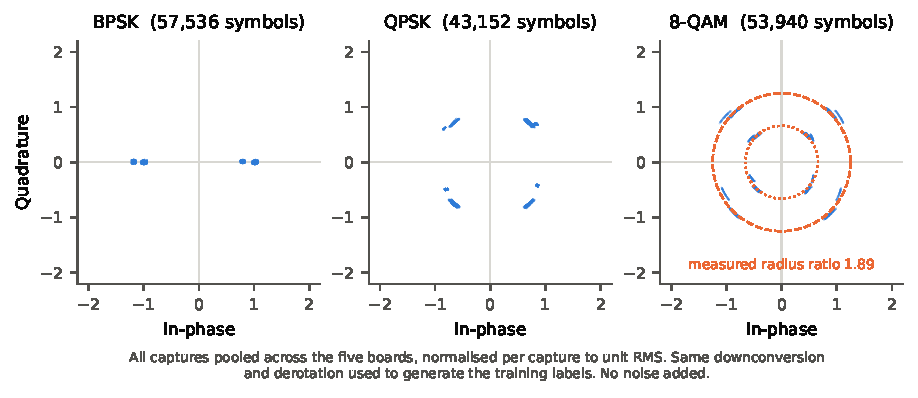
\includegraphics[width=\textwidth]{fig_constellation.pdf}
\caption{Measured constellations, all records pooled across the five boards and
normalised per record to unit RMS. The 8-QAM panel shows the two rings at the
measured radius ratio of $1.89$. No noise has been added.}
\label{fig:constellation}
\end{figure*}

% =====================================================================
\section{Ground Truth}
\label{sec:groundtruth}

Labels are derived from the transmitted waveform, not from the transmitter's
configuration. Fig.~\ref{fig:pipeline} shows the two processing paths and their
separation.

\begin{figure*}[!t]
\centering
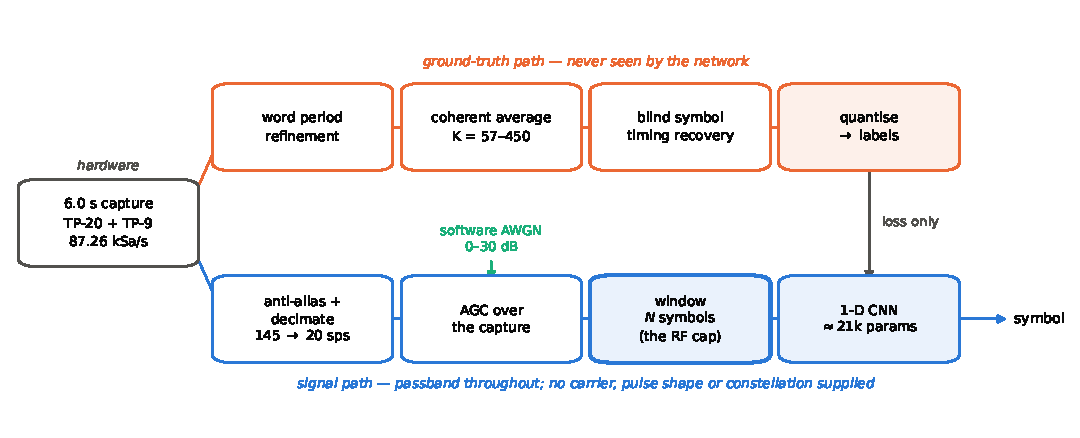
\includegraphics[width=\textwidth]{fig_pipeline.pdf}
\caption{Processing chain. The upper path produces ground-truth labels by
coherent averaging; the lower path produces the network's input. The paths share
only the raw capture, and the labels reach the network only through the loss.}
\label{fig:pipeline}
\end{figure*}

\subsection{Coherent averaging}
Let $x[n]$ be the captured passband waveform and $P$ the word period in samples,
which is not in general an integer. The record is folded into $K$ segments
resampled onto a common grid of $M = \lfloor P \rceil$ points,
\begin{equation}
x_k[m] = x\!\left(kP + m\tfrac{P}{M}\right),
\quad k = 0,\dots,K-1,
\label{eq:fold}
\end{equation}
and the template is their mean,
\begin{equation}
t[m] = \frac{1}{K}\sum_{k=0}^{K-1} x_k[m].
\label{eq:template}
\end{equation}
The period is refined by maximising the energy of the coherent average,
\begin{equation}
P^{\star} = \arg\max_{P} \ \operatorname{var}_m\big(t[m; P]\big),
\label{eq:period}
\end{equation}
searched over $\pm 6$ samples in steps of $0.02$ samples with $M$ held fixed so
that candidates are scored on a common grid. Writing
$\sigma_r^2 = \operatorname{var}(x_k[m] - t[m])$ for the residual variance, the
template signal-to-noise ratio is reported as
\begin{equation}
\mathrm{SNR}_t = 10\log_{10}
\frac{\operatorname{var}(t) - \sigma_r^2/K}{\sigma_r^2},
\label{eq:tsnr}
\end{equation}
in which the second numerator term removes the averaging bias, so the quantity
reported is the single-repetition signal-to-noise ratio rather than the
flattered post-averaging one.

\subsection{Symbol extraction}
The template is extended circularly before filtering, so that the final symbol
does not fall on the wrap boundary. Downconversion requires no external carrier
estimate: the word contains exactly $2N_s$ carrier cycles for $N_s$ symbols, so
\begin{equation}
b[n] = t_{\mathrm{ext}}[n] \, e^{-j 2\pi (2N_s) n / M},
\label{eq:downconv}
\end{equation}
which is exact regardless of the sample rate. After matched filtering, symbols
are sampled at instants $(i + \tau)T_s$, where the timing offset $\tau \in [0,1)$
is recovered blind by maximising mean symbol energy,
\begin{equation}
\tau^{\star} = \arg\max_{\tau} \ \frac{1}{N_s}\sum_{i} \big| s_i(\tau) \big|^2 .
\label{eq:timing}
\end{equation}
The residual constellation rotation is removed by an $m$th-power estimate,
\begin{equation}
\rho = \frac{1}{m}\arg\!\left(
  \mathbb{E}\!\left[s^m\right] e^{-j m \phi_{\mathrm{ref}}}\right),
\qquad s' = s\,e^{-j\rho},
\label{eq:derotate}
\end{equation}
with $m = 2$ for BPSK and $m = 4$ otherwise. The rotation must be applied inside
the argument as written: for a reference phase of $45^{\circ}$ the fourth-power
sum lies near $180^{\circ}$, on the branch cut of the argument function, and
subtracting afterwards places records whose phase is physically identical
$90^{\circ}$ apart. The estimate is taken over all $\approx3600$ symbols of the
record rather than over the symbols of one word, because a word covering the
constellation unevenly biases it enough to select a different quadrant. Either
error relabels every symbol of the affected record while leaving all per-record
diagnostics intact.

Symbol-timing recovery is a prerequisite rather than a refinement. Extracting
symbols without \eqref{eq:timing} places decision instants part-way through
transitions and collapses individual constellation radii---in our data, two of
the eight 8-QAM radii fell to $0.20$ against a nominal $1.31$. This artefact is
visually indistinguishable from a template wrap-boundary error and must be
excluded before that diagnosis is reached.

\subsection{Verification of the labels}
Two independent checks confirm the recovered labels.

\begin{enumerate}
\item All sixteen BPSK records reproduce the board's 63-bit maximal-length
sequence at $100\%$, against a chance level of $66.6\%$ (95th percentile
$69.8\%$) computed over 63 rotations and both polarities. The carrier is
recovered blind by fourth-power estimation at $1199.915$--$1199.918$~Hz across
all five boards.
\item A single memoryless bijection from constellation point to dibit fits all
three QPSK data words simultaneously at $100\%$---36 symbols explained by one
four-point mapping. Across $20{,}000$ label permutations preserving the
per-symbol occupancy counts, a perfect fit never occurred, giving
$p < 5\times10^{-5}$.
\end{enumerate}

The second check also resolves, for BPSK and QPSK, the mapping between
transmitter configuration and transmitted symbol. For 8-QAM it cannot: a word
covering all eight points exactly once admits a perfect bijection for any
rotation, so the test is vacuous for a single word and remains unresolved.

% =====================================================================
\section{Receiver}

\subsection{The receptive-field bound}
\label{sec:bound}
The transmitted sequence is a maximal-length sequence of linear order six,
satisfying
\begin{equation}
s[i+6] = s[i] \oplus s[i+5],
\label{eq:lfsr}
\end{equation}
so any six consecutive bits determine the seventh exactly. No five consecutive
bits do: each five-bit window occurs twice per period with distinct
successors~\cite{golomb1982shift}.

Consequently a receiver whose input contains at most five bits cannot predict a
symbol from its neighbours, and must extract it from the waveform. We enforce
this through the \emph{input} rather than through the layer stack: the network
receives a window of exactly $N$ symbols and labels the symbol within it, and
cannot attend to a sixth bit because no sixth bit is present in its input. The
formulation is verifiable by inspection and is unaffected by later changes to
the architecture. Table~\ref{tab:bound} gives the resulting configuration.

\begin{table}[!t]
\caption{Receptive-field bound and model size. All configurations remain at or
below the five-bit limit implied by \eqref{eq:lfsr}.}
\label{tab:bound}
\centering
\begin{tabular}{lrrrrr}
\toprule
Modulation & Symbols & Bits & Window & RF & Parameters \\
\midrule
BPSK  & 5 & 5 & 100 & 93 & 20{,}932 \\
QPSK  & 2 & 4 &  40 & 39 & 22{,}022 \\
8-QAM & 1 & 3 &  20 & 20 & 20{,}106 \\
\bottomrule
\end{tabular}
\end{table}

For a stack of one-dimensional convolutions with kernel sizes $k_l$ and strides
$s_l$, the receptive field in input samples is
\begin{equation}
\mathrm{RF} = 1 + \sum_{l} (k_l - 1)\prod_{j<l} s_j ,
\label{eq:rf}
\end{equation}
and is asserted against the window width in code. The bound is tightest for
8-QAM, where a single symbol already carries three bits; this is the
configuration in which the argument is weakest, and accordingly the one for
which we provide the largest number of independent held-out words.

\subsection{Signal conditioning}
Waveforms are low-pass filtered with a zero-phase FIR and decimated from
$145.44$ to $20$ samples per symbol, and are presented in \emph{passband}.
Conversion to baseband is not performed, as it would amount to supplying the
carrier frequency.

Amplitude is normalised by an automatic gain control computed over the whole
record,
\begin{equation}
\tilde{x}[n] = x[n] \big/ \sqrt{\textstyle\frac{1}{L}\sum_{l} x[l]^2 } ,
\label{eq:agc}
\end{equation}
which removes device gain---one board's output is $40\%$ below the
others---and attenuator setting, while preserving symbol-to-symbol amplitude
ratios. Per-window normalisation must not be used. An 8-QAM window is a single
symbol, and forcing it to unit energy erases the inner/outer ring distinction,
which carries one of the three bits per symbol; in our measurements this held
8-QAM symbol error rate at $0.50$ with no improvement from $0$~dB to noiseless,
because the ring bit was pure guesswork.

Additive white Gaussian noise is applied during training with the
signal-to-noise ratio drawn uniformly from $0$ to $30$~dB, referenced to the
record level of \eqref{eq:agc} so that all symbols in a record experience the
same noise power. Referencing to the individual window would give inner-ring
symbols less noise than outer-ring symbols, which no physical channel does.

\subsection{Architecture and objective}
The receiver is a four-layer one-dimensional convolutional network with 32
channels, a full-width learned combiner in place of global pooling, and two
output heads: symbol-class logits and a latent $(\hat{I},\hat{Q})$ pair. Global
average pooling was deliberately avoided: it makes the effective receptive field
equal to the whole input while a kernel-based calculation reports a smaller
figure, so the number one would quote would not be the operative one.

The training objective is
\begin{equation}
\mathcal{L} = \mathcal{L}_{\mathrm{CE}}
  + \lambda \min_{c \in \mathcal{C}}
    \big\lVert (\hat{I},\hat{Q}) - c \big\rVert^2 ,
\label{eq:loss}
\end{equation}
where $\mathcal{C}$ is the measured constellation of
Fig.~\ref{fig:constellation}: two antipodal points for BPSK, a single ring of
four for QPSK, and a two-ring star of radius ratio $1.89$ for 8-QAM.
Cross-entropy is class-weighted to compensate the intrinsic imbalance of the
transmitted words. Optimisation uses Adam at $2\times10^{-3}$ with cosine decay
over 25 epochs and a batch size of 512.

\subsection{Evaluation splits}
Partitions are constructed at \emph{record} level. Symbols within one record are
repetitions of a single data word through a single signal path, so a
symbol-level partition would place near-duplicates on both sides. Four splits
are reported: leave-one-pattern-out, leave-one-board-out,
leave-one-attenuation-out, and a random $80/20$ partition, the last included
explicitly as the optimistic reference. Thirty-five folds are evaluated in
total.

% =====================================================================
\section{Results}

\subsection{Error rate against a blind classical receiver}
\label{sec:ser}
The reference receiver performs fourth-power carrier recovery, matched filtering
and hard decision, and is given no parameter the network is not given. Noise is
identical for both. Fig.~\ref{fig:ser} and Table~\ref{tab:ser} report
leave-one-pattern-out performance.

\begin{figure*}[!t]
\centering
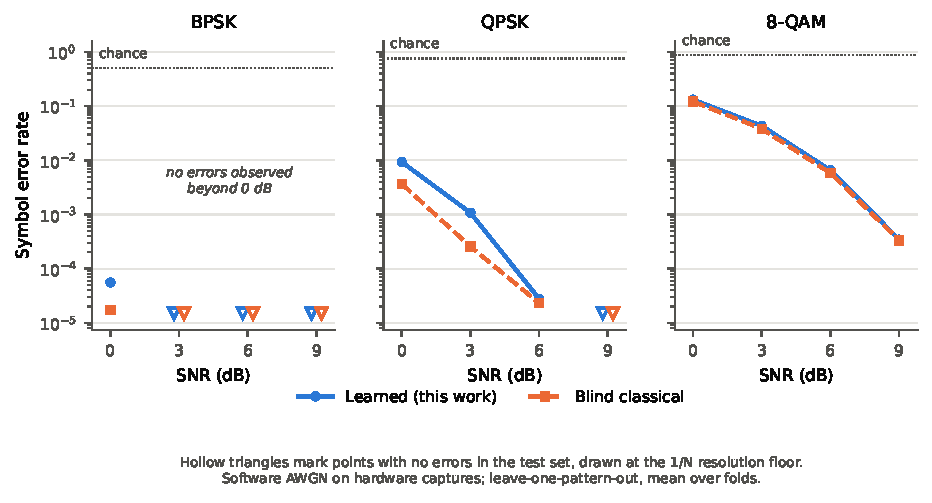
\includegraphics[width=\textwidth]{fig1_ser_vs_snr.pdf}
\caption{Symbol error rate against signal-to-noise ratio for the learned and
blind classical receivers, leave-one-pattern-out. Hollow triangles mark
operating points at which no errors occurred in the test set, drawn at the
$1/N$ resolution floor. All quantities saturate above $9$~dB.}
\label{fig:ser}
\end{figure*}

\begin{table}[!t]
\caption{Symbol error rate, learned (L) and blind classical (C) receivers,
leave-one-pattern-out, mean over folds.}
\label{tab:ser}
\centering
\begin{tabular}{lcccccc}
\toprule
& \multicolumn{2}{c}{BPSK} & \multicolumn{2}{c}{QPSK}
& \multicolumn{2}{c}{8-QAM} \\
\cmidrule(lr){2-3}\cmidrule(lr){4-5}\cmidrule(lr){6-7}
SNR & L & C & L & C & L & C \\
\midrule
$0$~dB & 0.0001 & 0.0000 & 0.0093 & 0.0037 & 0.1319 & 0.1219 \\
$3$~dB & 0.0000 & 0.0000 & 0.0011 & 0.0003 & 0.0432 & 0.0381 \\
$6$~dB & 0.0000 & 0.0000 & 0.0000 & 0.0000 & 0.0065 & 0.0058 \\
$9$~dB & 0.0000 & 0.0000 & 0.0000 & 0.0000 & 0.0003 & 0.0003 \\
\bottomrule
\end{tabular}
\end{table}

The two receivers are equivalent. The classical receiver retains a small
advantage at $0$~dB---$0.1219$ against $0.1319$ for 8-QAM, a relative difference
of $8\%$---which is expected, as a matched filter is near-optimal for additive
Gaussian noise. Above $9$~dB the learned receiver reaches zero errors while the
classical receiver retains a residual floor of $2\times10^{-4}$. We interpret
neither difference as a performance claim.

\subsection{Generalisation}
\label{sec:generalisation}

\begin{table}[!t]
\caption{8-QAM symbol error rate by evaluation split, mean over folds.}
\label{tab:splits}
\centering
\begin{tabular}{lccccc}
\toprule
Split & Folds & $0$~dB & $3$~dB & $6$~dB & $9$~dB \\
\midrule
Random $80/20$            & 1 & 0.1269 & 0.0387 & 0.0054 & 0.0005 \\
Leave-one-pattern-out     & 5 & 0.1319 & 0.0432 & 0.0065 & 0.0003 \\
Leave-one-board-out       & 5 & 0.1327 & 0.0451 & 0.0105 & 0.0021 \\
Leave-one-atten.-out & 2 & 0.1367 & 0.0452 & 0.0071 & 0.0004 \\
\bottomrule
\end{tabular}
\end{table}

Holding out an entire data word costs essentially nothing. At $0$~dB the
leave-one-pattern-out and random splits differ by $0.005$ in symbol error rate,
within run-to-run variation (Fig.~\ref{fig:splits}). This is the empirical
counterpart of the bound of Section~\ref{sec:bound}: a model exploiting sequence
structure would score markedly better on a random split, in which training and
test partitions share the same data word. It does not.

Cross-device transfer is measurably harder. Leave-one-board-out degrades to
$0.0021$ at $9$~dB against $0.0003$ for leave-one-pattern-out, a factor of
seven. The effect is small in absolute terms but consistent across folds, and is
the only split exhibiting a systematic gap.

\begin{figure}[!t]
\centering
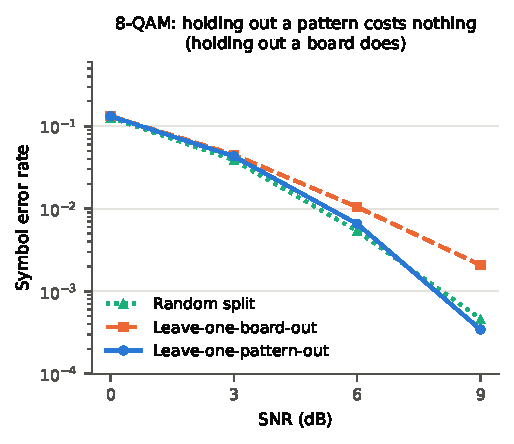
\includegraphics[width=\columnwidth]{fig2_no_memorisation.pdf}
\caption{8-QAM symbol error rate by evaluation split. Withholding a complete
data word is indistinguishable from a random partition; withholding a board is
not.}
\label{fig:splits}
\end{figure}

Per-fold results are given in Table~\ref{tab:perfold}. Two folds are thin and
are reported with their training size: BPSK with the pseudorandom sequence held
out trains on a single record and QPSK with its primary word held out trains on
two. The 8-QAM folds, where the bound of Section~\ref{sec:bound} is tightest,
are the best conditioned: four of five train on fourteen records.

% Seven columns do not fit one column of a two-column layout (73pt over).
% Promoted to a full-width float rather than shrinking the type further.
\begin{table*}[!t]
\caption{Per-fold results. \emph{Train rec.} is the number of records in the
training partition; the two folds with fewer than three are the thin folds
discussed in the text. \emph{Position-only} is a lookup from a symbol's index
within the data word to its most frequent label, against chance levels of
$0.500$, $0.750$ and $0.875$. It is a meaningful control only where the withheld
word is absent from training; every leave-one-board-out fold reuses the training
word, position then determines the label exactly, and the entry is marked
\textit{n/a} (Section~\ref{sec:controls}).
}

\label{tab:perfold}
\centering
\begin{tabular}{llrrrrr}
\toprule
Modulation & Held out & Train records & Test symbols
& SER at $0$~dB & SER at $6$~dB & Position-only \\
\midrule
\textit{Leave-one-pattern-out} & & & & & & \\
BPSK & PRBS63 & 1 & 53{,}880 & 0.0001 & 0.0000 & 0.5290 \\
BPSK & S1 & 15 & 3{,}592 & 0.0000 & 0.0000 & 0.5003 \\
QPSK & Q1 & 2 & 35{,}950 & 0.0174 & 0.0001 & 0.7751 \\
QPSK & Q2 & 11 & 3{,}595 & 0.0042 & 0.0000 & 0.7502 \\
QPSK & Q3 & 11 & 3{,}595 & 0.0064 & 0.0000 & 0.8334 \\
8-QAM & T1+T2 & 4 & 39{,}556 & 0.1519 & 0.0119 & 0.8864 \\
8-QAM & T3 & 14 & 3{,}596 & 0.1310 & 0.0072 & 0.8749 \\
8-QAM & T4 & 14 & 3{,}596 & 0.1313 & 0.0028 & 0.7500 \\
8-QAM & T5 & 14 & 3{,}596 & 0.1271 & 0.0044 & 0.8751 \\
8-QAM & T6 & 14 & 3{,}596 & 0.1185 & 0.0064 & 0.8751 \\
\addlinespace
\textit{Leave-one-board-out} & & & & & & \\
BPSK & B1 & 12 & 14{,}368 & 0.0001 & 0.0000 & n/a \\
BPSK & B2 & 13 & 10{,}776 & 0.0000 & 0.0000 & n/a \\
BPSK & B3 & 13 & 10{,}776 & 0.0002 & 0.0000 & n/a \\
BPSK & B4 & 13 & 10{,}776 & 0.0000 & 0.0000 & n/a \\
BPSK & B5 & 13 & 10{,}776 & 0.0002 & 0.0000 & n/a \\
QPSK & B1 & 8 & 14{,}380 & 0.0070 & 0.0000 & n/a \\
QPSK & B2 & 10 & 7{,}190 & 0.0054 & 0.0000 & n/a \\
QPSK & B3 & 10 & 7{,}190 & 0.0049 & 0.0000 & n/a \\
QPSK & B4 & 10 & 7{,}190 & 0.0036 & 0.0000 & n/a \\
QPSK & B5 & 10 & 7{,}190 & 0.0174 & 0.0001 & n/a \\
8-QAM & B1 & 8 & 25{,}172 & 0.1287 & 0.0057 & n/a \\
8-QAM & B2 & 13 & 7{,}192 & 0.1194 & 0.0049 & n/a \\
8-QAM & B3 & 13 & 7{,}192 & 0.1193 & 0.0057 & n/a \\
8-QAM & B4 & 13 & 7{,}192 & 0.1283 & 0.0060 & n/a \\
8-QAM & B5 & 13 & 7{,}192 & 0.1675 & 0.0302 & n/a \\
\bottomrule
\end{tabular}
\end{table*}

\subsection{Negative controls}
\label{sec:controls}
\begin{table}[!t]
\caption{Controls, leave-one-pattern-out folds. Both must fail, and both do.
The position-only control is restricted to this split for the reason given in
the text.}
\label{tab:controls}
\centering
\begin{tabular}{lcccc}
\toprule
Modulation & Chance & Shuffled & Position-only & Model \\
\midrule
BPSK  & 0.500 & 0.4979 & 0.5147 & 0.0000 \\
QPSK  & 0.750 & 0.7349 & 0.7862 & 0.0000 \\
8-QAM & 0.875 & 0.8834 & 0.8523 & 0.0065 \\
\bottomrule
\end{tabular}
\end{table}

Permuting labels among the symbols of each fold leaves performance at chance,
confirming that no path exists from input to target other than the waveform.

The second control requires a qualification that is easy to overlook. Labels are
a periodic tiling of the transmitted word, so a symbol's index within that word
determines its label exactly. Across all $148$ pairs of records carrying the same
word---including pairs drawn from different boards and different
attenuations---the label sequences are identical up to a cyclic shift. A
predictor reading only the symbol index therefore attains a symbol error rate of
zero on any split whose test partition reuses a training word, which is the case
for every leave-one-board-out, leave-one-attenuation-out and random fold. On
those splits the position-only figure is not a control and we do not report it.

It is a control on leave-one-pattern-out, where the withheld word is absent from
training and is not a cyclic shift of any training word: the best cyclic
agreement between distinct words is $0.500$ for QPSK and $0.375$ for 8-QAM,
against chance agreements of $0.250$ and $0.125$. There the lookup sits at
chance for all three modulations---$0.5147$ against $0.500$, $0.7862$ against
$0.750$, and $0.8523$ against $0.875$ (Table~\ref{tab:controls},
Fig.~\ref{fig:controls}).

This concerns the control, not the receiver. The network is given a window of
waveform samples and nothing else: it receives no symbol index and classifies
each window independently, so on no split can it exploit the positional
redundancy that defeats the lookup.

\begin{figure}[!t]
\centering
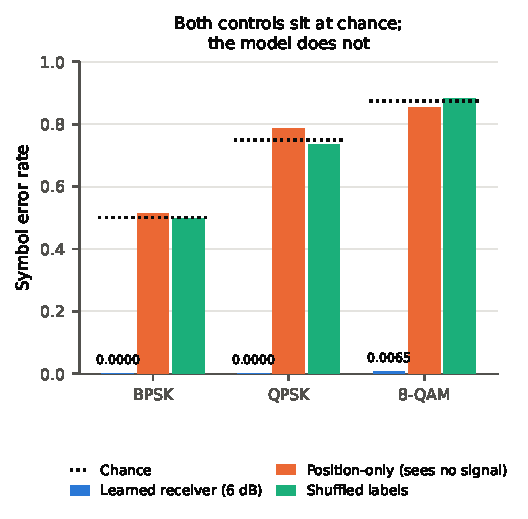
\includegraphics[width=\columnwidth]{fig3_controls.pdf}
\caption{Both negative controls remain at their respective chance levels while
the receiver does not. Leave-one-pattern-out folds.}
\label{fig:controls}
\end{figure}

\subsection{Recovered constellation geometry}
\label{sec:geometry}
The constellation term of \eqref{eq:loss} was ablated across two decades of
$\lambda$ (Table~\ref{tab:ablation}). \emph{The constellation prior does not
improve error rate.} Its role is interpretability: it aligns the latent
$(\hat{I},\hat{Q})$ head with the physical constellation. We do not present it as
a performance mechanism.

\begin{table}[!t]
\caption{Ablation of the constellation term of \eqref{eq:loss},
leave-one-board-out. Differences lie within run-to-run variation.}
\label{tab:ablation}
\centering
\begin{tabular}{lcccc}
\toprule
& \multicolumn{3}{c}{8-QAM} & QPSK \\
\cmidrule(lr){2-4}\cmidrule(lr){5-5}
$\lambda$ & $0$~dB & $3$~dB & $6$~dB & $0$~dB \\
\midrule
$0.0$ & 0.1246 & 0.0370 & 0.0060 & 0.0058 \\
$0.2$ & 0.1261 & 0.0359 & 0.0056 & 0.0051 \\
$1.0$ & 0.1276 & 0.0364 & 0.0058 & 0.0054 \\
\bottomrule
\end{tabular}
\end{table}

The geometry is nevertheless recovered, by the classifier alone and from data.
Examining the destination of errors at $0$~dB (Fig.~\ref{fig:geometry}),
$79.5\%$ of 8-QAM errors land on the geometrically nearest constellation point
against a chance level of $14.3\%$, an enrichment of $5.6\times$; for QPSK the
corresponding figures are $100\%$ against $66.7\%$. Of the 56 off-diagonal cells
of the confusion matrix, 36 are exactly zero, and the populated cells are the
same-phase ring transition and the adjacent-quadrant transition---the two
shortest distances in the constellation.

A receiver implementing a memorised waveform-to-label mapping would distribute
errors uniformly over incorrect classes. This one confuses each point with its
metric neighbours, which is where additive noise transports a symbol.

\begin{figure*}[!t]
\centering
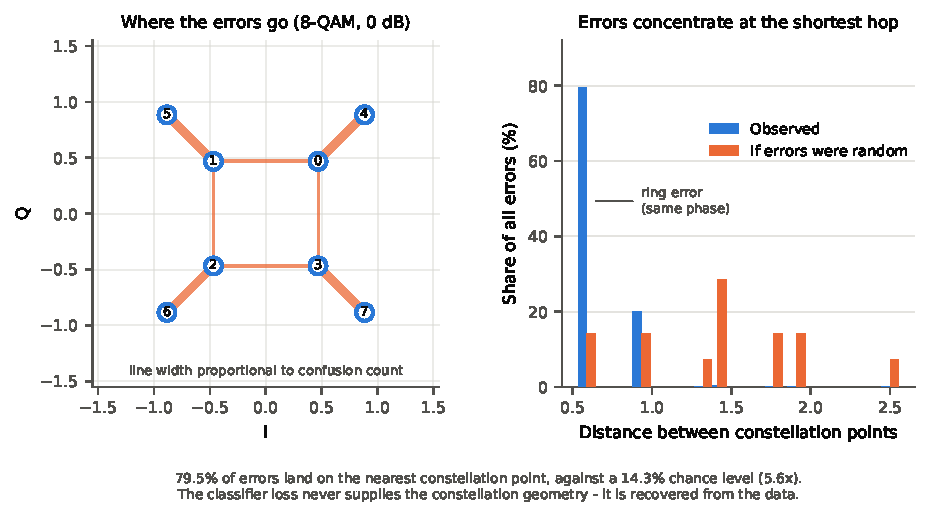
\includegraphics[width=\textwidth]{fig5_error_geometry.pdf}
\caption{Destination of 8-QAM errors at $0$~dB. Left: confusions drawn on the
constellation, line width proportional to count. Right: share of errors against
inter-point distance, compared with a uniform-error null.}
\label{fig:geometry}
\end{figure*}

\subsection{Hardware characterisation}
\label{sec:hardware}
The captures also characterise the boards' own demodulators, measured against
the known transmitted sequence rather than by self-consistency
(Fig.~\ref{fig:lock}). Across all five units, agreement with the transmitted
sequence is at chance for every record below $509$~mV output level and reaches
$92$--$100\%$ for every record above $626$~mV. A single threshold within that
interval accounts for all five boards.

\begin{figure}[!t]
\centering
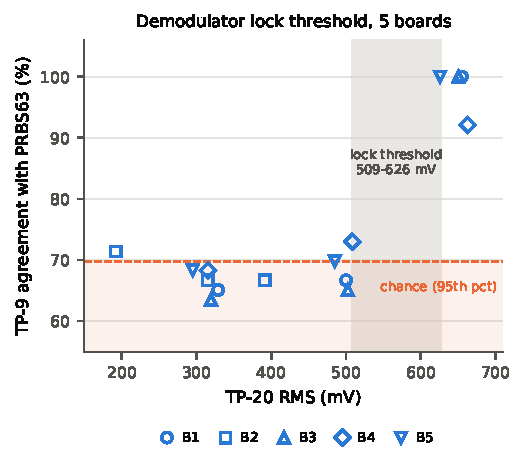
\includegraphics[width=\columnwidth]{fig4_lock_threshold.pdf}
\caption{Demodulator lock threshold across five boards, measured against the
known transmitted sequence. A single threshold accounts for every unit.}
\label{fig:lock}
\end{figure}

Board-level behaviour differs in kind rather than degree. One board's BPSK path
delivers $391$~mV where the others deliver $626$--$663$~mV and never reaches
threshold, while its QPSK and 8-QAM outputs are indistinguishable from the
others (cross-board waveform correlation $+0.9987$ and $+0.9991$, against
$+0.9769$ for BPSK). A second board crosses the threshold but locks
imperfectly, at $92.1\%$.

We recommend against self-consistency as a lock criterion. A demodulator that
has lost lock also repeats. On one board at $329$~mV, self-consistency read
$0.979$ while agreement with the transmitted sequence was at chance: the
unlocked demodulator had entered a stable period-two state, inverting its output
every word period (autocorrelation $-0.93$ at one word period, $+0.90$ at two).
Four records in this study would have been misclassified as locked by that
metric.

Finally, the boards' own QPSK demodulator failed to lock on the primary QPSK
word on all five units, at both attenuator settings, although the fingerprint
check confirms the word was correctly loaded. No hardware baseline is therefore
available for QPSK.

% =====================================================================
\section{Discussion}

\subsection{Evaluation validity as the primary result}
The principal result of this work is methodological. When a learned receiver is
trained on a periodic transmitted sequence, held-out evaluation alone does not
establish that the receiver demodulates. The property can instead be guaranteed:
by bounding the receiver's input below the linear order of the transmitted
sequence, prediction-from-context becomes impossible rather than unlikely, and
the guarantee survives any change to model capacity or training procedure.

That guarantee has an empirical signature---no gap between a random partition
and a leave-one-pattern-out partition---which is then available as a consistency
check rather than as the primary evidence. We observe that signature
(Section~\ref{sec:generalisation}). The two lines of argument are independent:
the bound would hold even had the gap been large, and the small gap would be
suggestive but not conclusive without the bound.

We note that the bound is cheap to adopt. It requires knowing the linear order
of the transmitted sequence, which is a property of the test signal rather than
of the receiver, and constraining the input window accordingly. Where a test
sequence has high linear complexity the constraint is loose; where it is a short
m-sequence, as in much laboratory practice, it is tight and necessary.

\subsection{Interpreting parity}
The parity result of Section~\ref{sec:ser} should be read in this light. A
matched-filter receiver with correct carrier recovery is near-optimal for the
channel studied here, and a learned receiver cannot be expected to exceed it.
The substantive observation is that parity is reached without supplying the
carrier frequency, the pulse shape, the constellation geometry or the decision
boundaries, and that the constellation is recovered from data with a $5.6\times$
enrichment toward nearest-neighbour errors.

The one systematic gap we observe is cross-device: leave-one-board-out is
consistently worse than leave-one-pattern-out at high signal-to-noise ratio.
This is the expected direction---the boards differ measurably in output level,
constellation tightness and transmit-filter delay---and it suggests that
device-invariant training, rather than sequence generalisation, is where the
remaining headroom lies for this class of receiver.

\subsection{Implications for instrumentation practice}
The hardware characterisation of Section~\ref{sec:hardware} is of independent
interest to anyone evaluating aged laboratory equipment. That a demodulator
which has lost lock can present a perfectly self-consistent output is not, in
our experience, widely appreciated, and any protocol treating repeatability as
evidence of correct operation is exposed to it. The failure is also invisible on
an oscilloscope: an unlocked digital output looks entirely normal at any time
base. We therefore recommend that lock be established only by comparison against
a known transmitted sequence.

% =====================================================================
\section{Limitations}
\label{sec:limitations}

\emph{Content diversity.} The corpus is large in noise realisations and hardware
variation but small in distinct transmitted content: 8-QAM comprises five
independent 24-bit words, or 40 distinct symbol instances.

\emph{Device count.} Five functional units support a five-fold cross-device
evaluation. The device-to-device differences we observe are large enough to be
measured but the sample is too small to characterise their distribution.

\emph{Synthetic noise.} The hardware supplies the waveform---carrier, filter
response, quantisation, device-to-device variation---while additive white
Gaussian noise is applied in software. The boards' own noise control contributes
approximately $+0.02$~dB within the signal band and is unusable as a
signal-to-noise axis.

\emph{Symbol timing is supplied.} The receiver is given neither the carrier
frequency nor the pulse shape, but its input window is symbol-synchronous, which
supplies the symbol rate and the sampling phase. This is not incidental: under a
one-symbol receptive field for 8-QAM, blind timing recovery is impossible, so
the receptive-field bound and timing-blindness cannot both hold. The system
should be described as operating on symbol-synchronous windows from a
conventional timing front-end~\cite{gardner1986ted}.

\emph{Carrier sensitivity does not support a robustness claim.} We measured
whether a classical receiver's dependence on carrier knowledge constitutes a
practical disadvantage. Estimating the carrier blind from eight symbols
($13.3$~ms) gives an error of $1.02$~Hz, yet demodulating those same eight
symbols with that estimate yields zero errors, because over $13.3$~ms a $1$~Hz
offset corresponds to $4.9^{\circ}$ of phase rotation. Estimate error and
tolerance contract together, and the classical receiver was self-consistent at
every observation length tested, from 8 to $3{,}596$ symbols. Reporting a
collapse under an externally imposed carrier offset would misrepresent a
receiver that does not make that error, and we therefore do not report one.

\emph{Operating regime.} A single carrier frequency, a single symbol rate, and
an additive Gaussian channel without multipath or fading. Generalisation beyond
this regime is not evidenced here.

% =====================================================================
\section{Conclusion}
We have presented a hardware dataset of 43 dual-channel captures from five
distinct communication trainer boards, together with a convolutional receiver
whose input is bounded below the linear order of the transmitted sequence, so
that sequence memorisation is excluded by construction rather than argued from
held-out performance. The receiver attains symbol error rates indistinguishable
from a blind matched-filter receiver across BPSK, QPSK and star 8-QAM while
receiving none of the parameters that receiver requires, and its errors
concentrate on nearest constellation neighbours at $5.6\times$ the chance rate,
indicating that the constellation geometry is recovered from the waveform. Two
negative results are reported: a constellation-geometry loss term does not
improve error rate, and a classical receiver's dependence on carrier knowledge
did not, under measurement, constitute a practical disadvantage.

Future work should address the two limitations that bound the present study
most tightly: the number of distinct transmitted words, which sets the
resolution of the leave-one-pattern-out evaluation, and the number of devices,
which sets the resolution of the cross-device evaluation.

% =====================================================================
\section*{Acknowledgment}
\todonote{acknowledgment}{%
Laboratory access, the technical assistance received during the capture
campaign, and any funding source. The lab assistant who supported the bench
sessions should be named here if not an author.}

\todonote{references --- VERIFY BEFORE SUBMISSION}{%
Every entry in \texttt{refs.bib} was written from working knowledge, not copied
from a database. Author lists, titles, venues and years are believed correct;
\textbf{volumes and page numbers must be checked} against IEEE Xplore, and DOIs
added. Delete this note once verified.}

\bibliographystyle{IEEEtran}
\bibliography{refs}

% =====================================================================
\todonote{author biographies}{%
IEEE Access requires a short biography and a photograph for each author, placed
here after the references. Use the \texttt{IEEEbiography} environment from the
class documentation; the photograph is passed as the optional argument as a
$1\,\text{in}\times1.25\,\text{in}$ \texttt{includegraphics} with
\texttt{keepaspectratio}.}

\end{document}
